%**************** TESTS FOR THE CODE ******************
\section{Tests on Synthetic Graphs}\label{sec5.2}
\subsection{Stochastic Block Model Test Graph}
To start testing our code we choose a Stochastic Block Model (SBM) graph. An SBM graph is a type of random graph model used to generate networks with a predefined community structure. It is an extension of the Erdos--R\'enyi, where nodes are divided into communities, and the probability of an edge between two nodes depends on their community membership. It is characterized by \textit{N} nodes, \textit{k} communities and a connectivity matrix \textit{$P_{ij}$} which represents the probability of an edge between a node in community $i$ and a node in community $j$.
Since communities are predefined when generating the graph, we can directly compare the detected communities with the true ones.

For our test we set 
\begin{equation*}
    N = 500, \quad k = 2, \quad
    P =
    \begin{bmatrix} 
        0.20 & 0.03 \\
        0.03 & 0.20
    \end{bmatrix}
\end{equation*}
with every initial weight equal to one.

Curvature values for the initial SBM graph are shown in fig.~\ref{fig:SBM_comparison_a}, while on the right we have the updated curvatures after 10 iterations of Ricci Flow. We can see that the community structure of this graph is already well established; Ricci Flow has however highlighted the weak connection of central inter community nodes as one can see in fig.~\ref{fig:SBM_comparison_b}.
\begin{figure}
    \centering
    \begin{subfigure}{0.45\textwidth}
        \centering
        \includegraphics[width=\textwidth]{../tests/ToyModelResults/SBM/Before Ricci Flow.png}
        \caption{Initial SBM graph, before Ricci Flow.}
        \label{fig:SBM_comparison_a}
    \end{subfigure}
    \hfill
    \begin{subfigure}{0.45\textwidth}
        \centering
        \includegraphics[width=\textwidth]{../tests/ToyModelResults/SBM/After Ricci Flow.png}
        \caption{SBM graph after Ricci Flow.}
        \label{fig:SBM_comparison_b}
    \end{subfigure}
    \caption{Comparison of SBM graph before and after having applied 10 iterations of Ricci Flow on edges.}
\end{figure}

In fig.~\ref{fig:SBM_Accuracy} we see that surgery with a cutoff between 1 and $\approx$1.5 leads to a perfect distinction between the two communities, i.e., an ARI of 1.

\begin{figure}
    \centering
    \includegraphics[width=0.6\textwidth]{../tests/ToyModelResults/SBM/Surgery Accuracy.png}
    \caption{SBM graph's ARI and modularity behaviour for different surgery cutoffs.}
    \label{fig:SBM_Accuracy}
\end{figure}

Lastly, fig.~\ref{fig:SBM_Communities_a} depicts the graph after surgery with a cutoff between 1 and $\approx$1.5. As expected, we got a separation into two distinct clusters. Fig.~\ref{fig:SBM_Communities_b} shows the two communities corresponding to the two connected components.
\begin{figure}
    \centering
    \begin{subfigure}{0.45\textwidth}
        \centering
        \includegraphics[width=\textwidth]{../tests/ToyModelResults/SBM/After Surgery.png}
        \caption{Final SBM graph, after surgery process.}
        \label{fig:SBM_Communities_a}
    \end{subfigure}
    \hfill
    \begin{subfigure}{0.45\textwidth}
        \centering
        
\includegraphics[width=\textwidth]{../tests/ToyModelResults/SBM/Detected Communities.png}
        \caption{Detected communities after surgery on SBM graph.}
        \label{fig:SBM_Communities_b}
    \end{subfigure}
    \caption{Comparison of SBM graph after surgery and corresponding connected components (i.e., the detected communities).}
\end{figure}


\subsection{Lancichinetti-Fortunato-Radicchi Test Graph}
As a more complex synthetic graph for testing we used a Lancichinetti-Fortunato-Radicchi (LFR) benchmark graph. LFR graphs are widely used for testing community-detection algorithms because they produce networks with heterogeneous (scale-free) degree distributions and community-size distributions, making them more realistic than simpler models. Nodes are assigned to communities according to specified power-law exponents, and a “mixing” parameter controls the fraction of edges that connect different communities.

For our test we built a graph with 500 nodes $\bigl(n = 500\bigr)$ with a degree distribution exponent $\tau_{1} = 3$ and a community-size exponent $\tau_{2} = 1.5$. For the mixing parameter we chose $\mu = 0.2$ indicates a relatively strong community structure by limiting the proportion of inter-community edges. We set each community to have a minimum of 20 nodes and a maximum of 70 nodes. The expected average degree is set to 20, with a maximum node degree capped at 50. 

For this graph we applied 40 iterations of Ricci Flow as its structure is more complex than the previous SBM graph (see fig.~\ref{fig:LFR_comparison_a}). In fig.~\ref{fig:LFR_comparison_b} we see a convergence of the curvature values after Ricci Flow; the high number of nodes and communities makes difficult to visualize properly the graph, for this reason we introduced also a histogram plot of weights and curvature values in the final code implementation for the Karate club graph (see \autoref{sec5.3}).
\begin{figure}
    \centering
    \begin{subfigure}{0.45\textwidth}
        \centering
        \includegraphics[width=\textwidth]{../tests/ToyModelResults/LFR/Before Ricci Flow.png}
        \caption{Initial LFR graph, before Ricci Flow.}
        \label{fig:LFR_comparison_a}
    \end{subfigure}
    \hfill
    \begin{subfigure}{0.45\textwidth}
        \centering
        \includegraphics[width=\textwidth]{../tests/ToyModelResults/LFR/After Ricci Flow.png}
        \caption{LFR graph after Ricci Flow.}
        \label{fig:LFR_comparison_b}
    \end{subfigure}
    \caption{Comparison of LFR graph before and after having applied 40 iterations of  Ricci Flow on edges.}
\end{figure}

Fig.~\ref{fig:LFR_Accuracy} shows the behaviour of ARI and modularity depending on the chosen cutoff point. Also in this case we see that it is possible to obtain an ARI of 1.
\begin{figure}
    \centering
    \includegraphics[width=0.6\textwidth]{../tests/ToyModelResults/LFR/Surgery Accuracy.png}
    \caption{LFR graph's ARI and modularity behaviour for different surgery cutoffs.}
    \label{fig:LFR_Accuracy}
\end{figure}

In fig.~\ref{fig:LFR_Surgery} we have the graph after surgery (we chose as cutoff $\approx$1.12 to get an ARI of 1) and we can see that it got divided into connected components with all the nodes of the same colour, i.e., same community. In this case we did not produce a plot community by community due to the high number of clusters. 
\begin{figure}
    \centering
    \includegraphics[width=0.6\textwidth]{../tests/ToyModelResults/LFR/After Surgery.png}
        \caption{Final LFR graph, after surgery process.}
        \label{fig:LFR_Surgery}
\end{figure}

\subsection{Additional Tests on Lancichinetti-Fortunato-Radicchi Graphs}
As a final test for our code we decided to try reproducing a result presented in the work of Ni et al. (see \textit{figure 8a} at page 12 of~\cite{Ni:communitydetectionnetworksricci}). In particular, it is about applying Ricci Flow on different LFR graphs differing for the modularity parameter $\mu$ and the average degree. Of course one expects the ARI to decrease with increasing values of $\mu$ as the community structure becomes less defined.

In fig.~\ref{fig:LFR_OTD} we present our results with OTD method for curvature evaluation. ARI decreases with increasing $\mu$ as expected and does not show significant differences between different values of average degree.
\begin{figure}
    \centering
    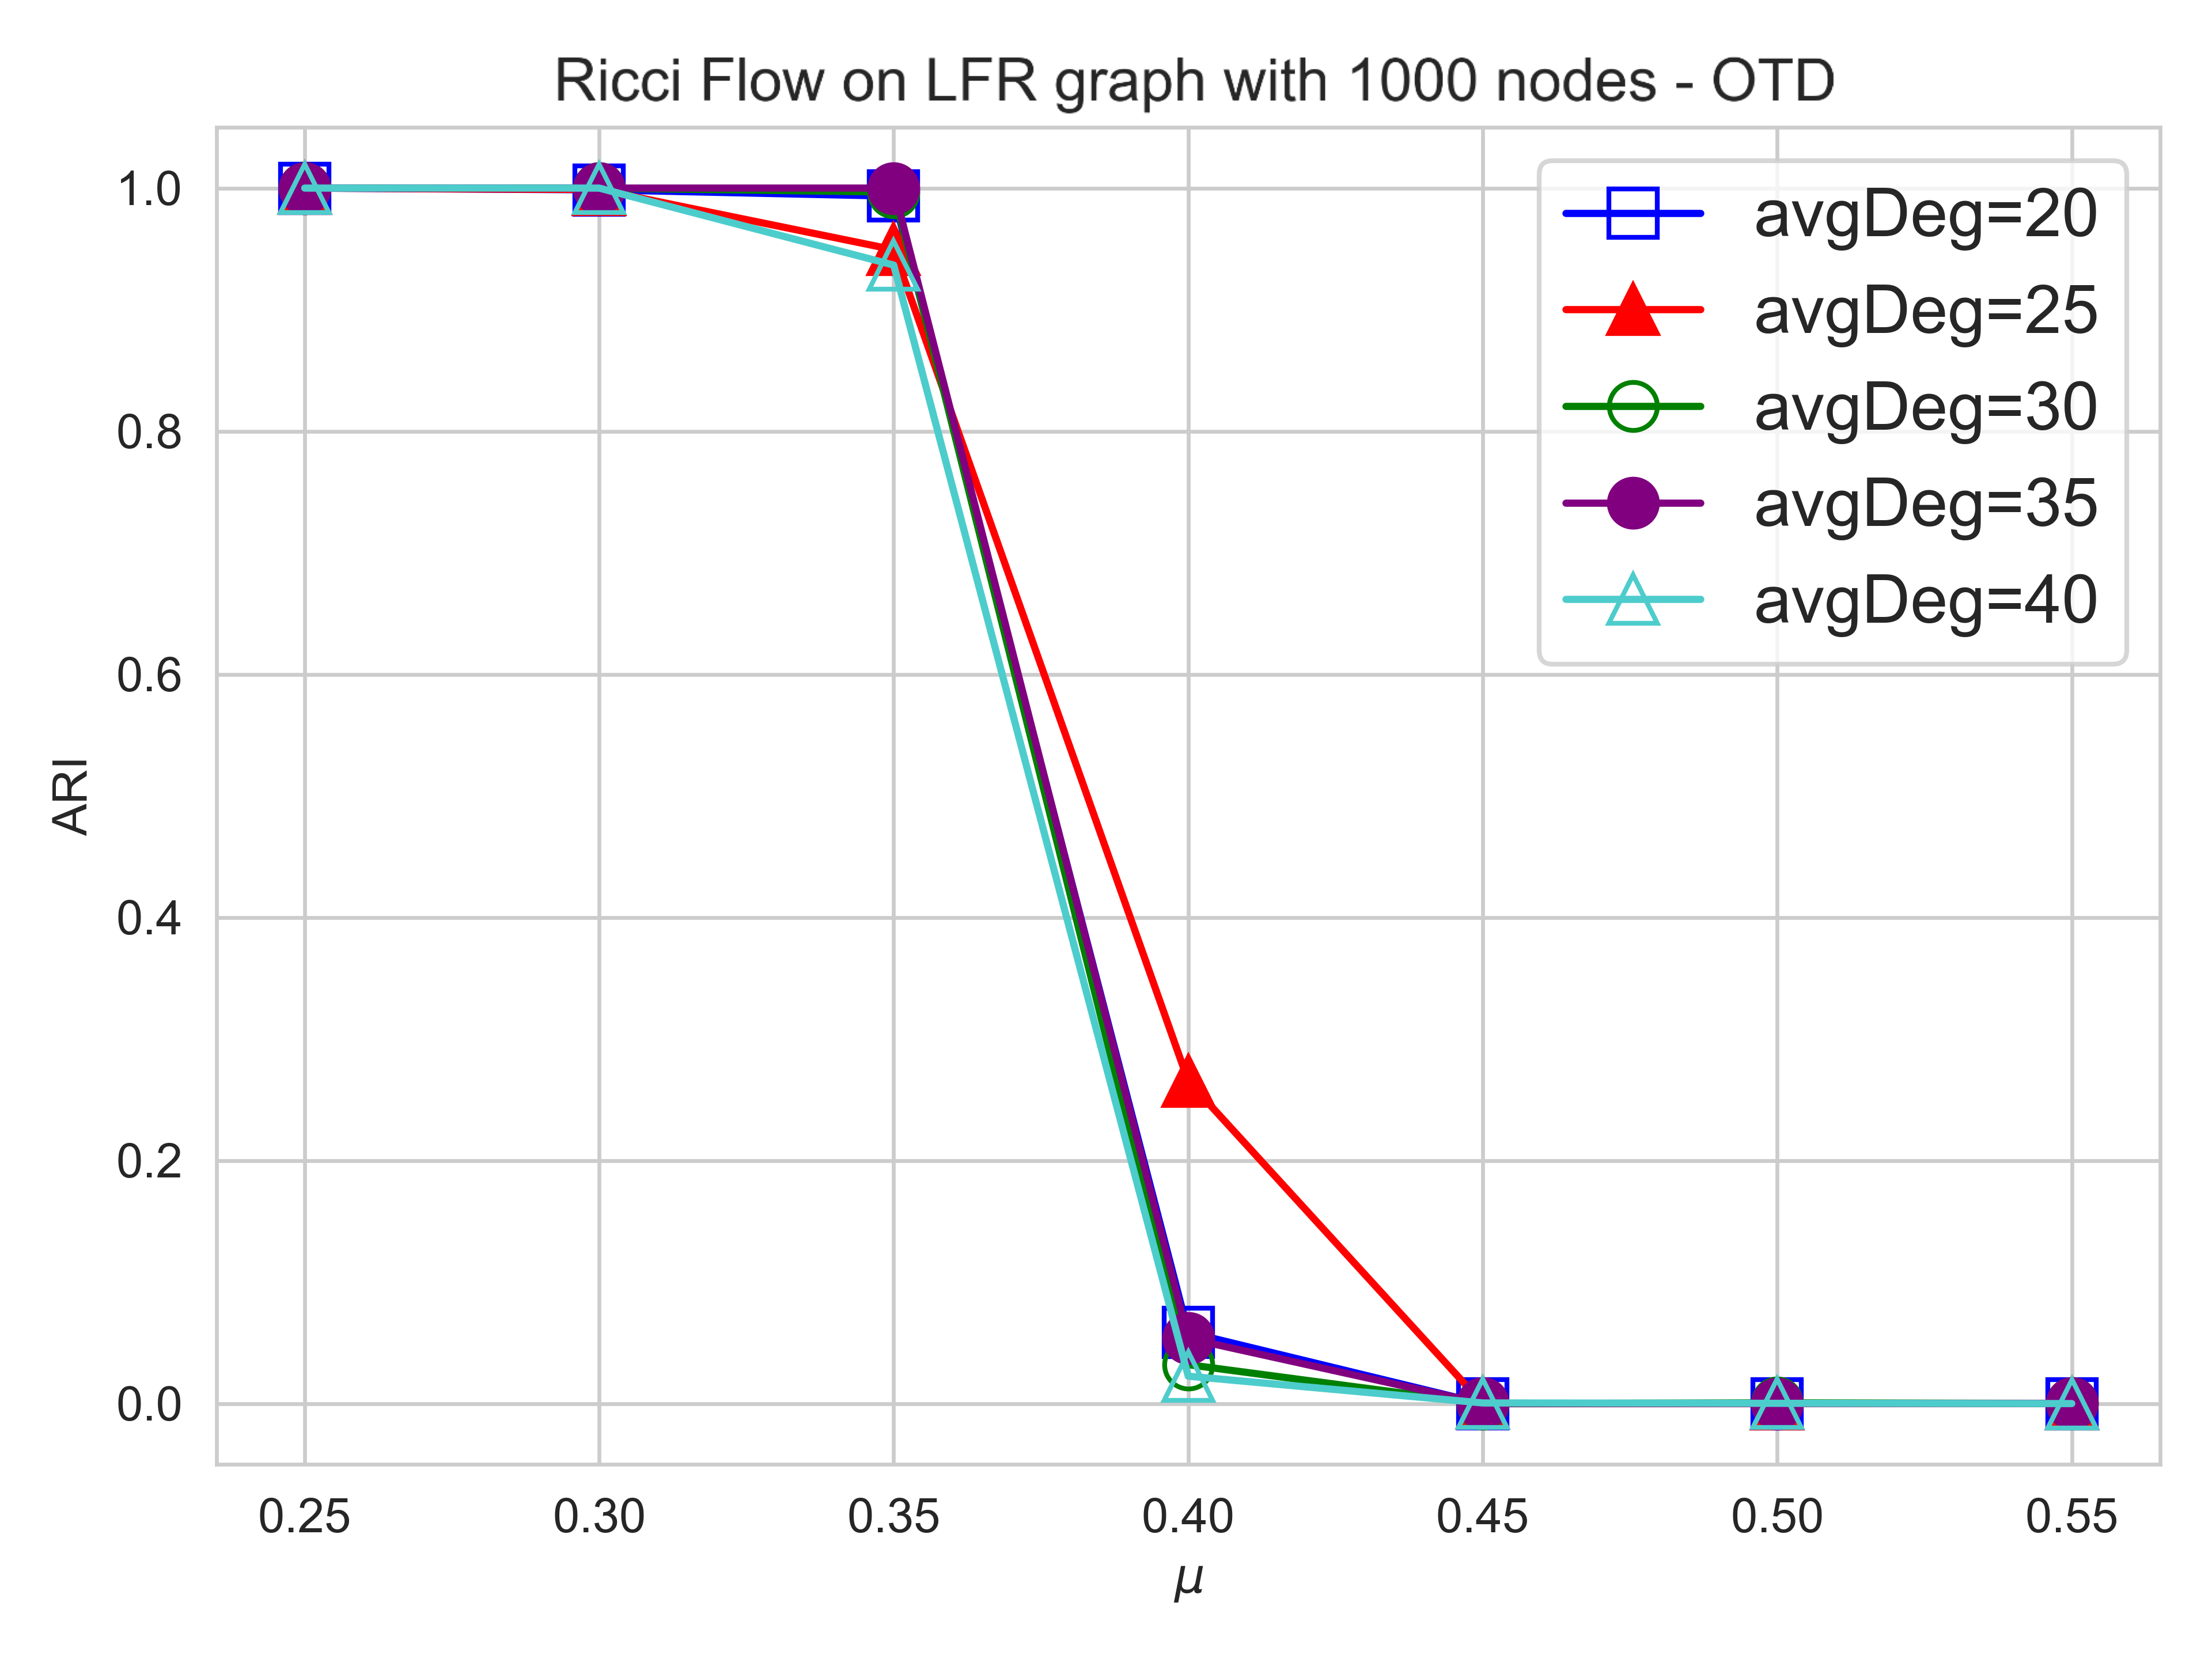
\includegraphics[width=0.6\textwidth]{../tests/LFRResults/LFR_OTD.png}
    \caption{LFR OTD}
    \label{fig:LFR_OTD}
\end{figure}

On the other hand, fig.~\ref{fig:LFR_ATD} shows a much poorer performance and the choice of the average degree seems to be more relevant. This is in accordance with ATD method being faster than OTD, but also less precise.
\begin{figure}
    \centering
    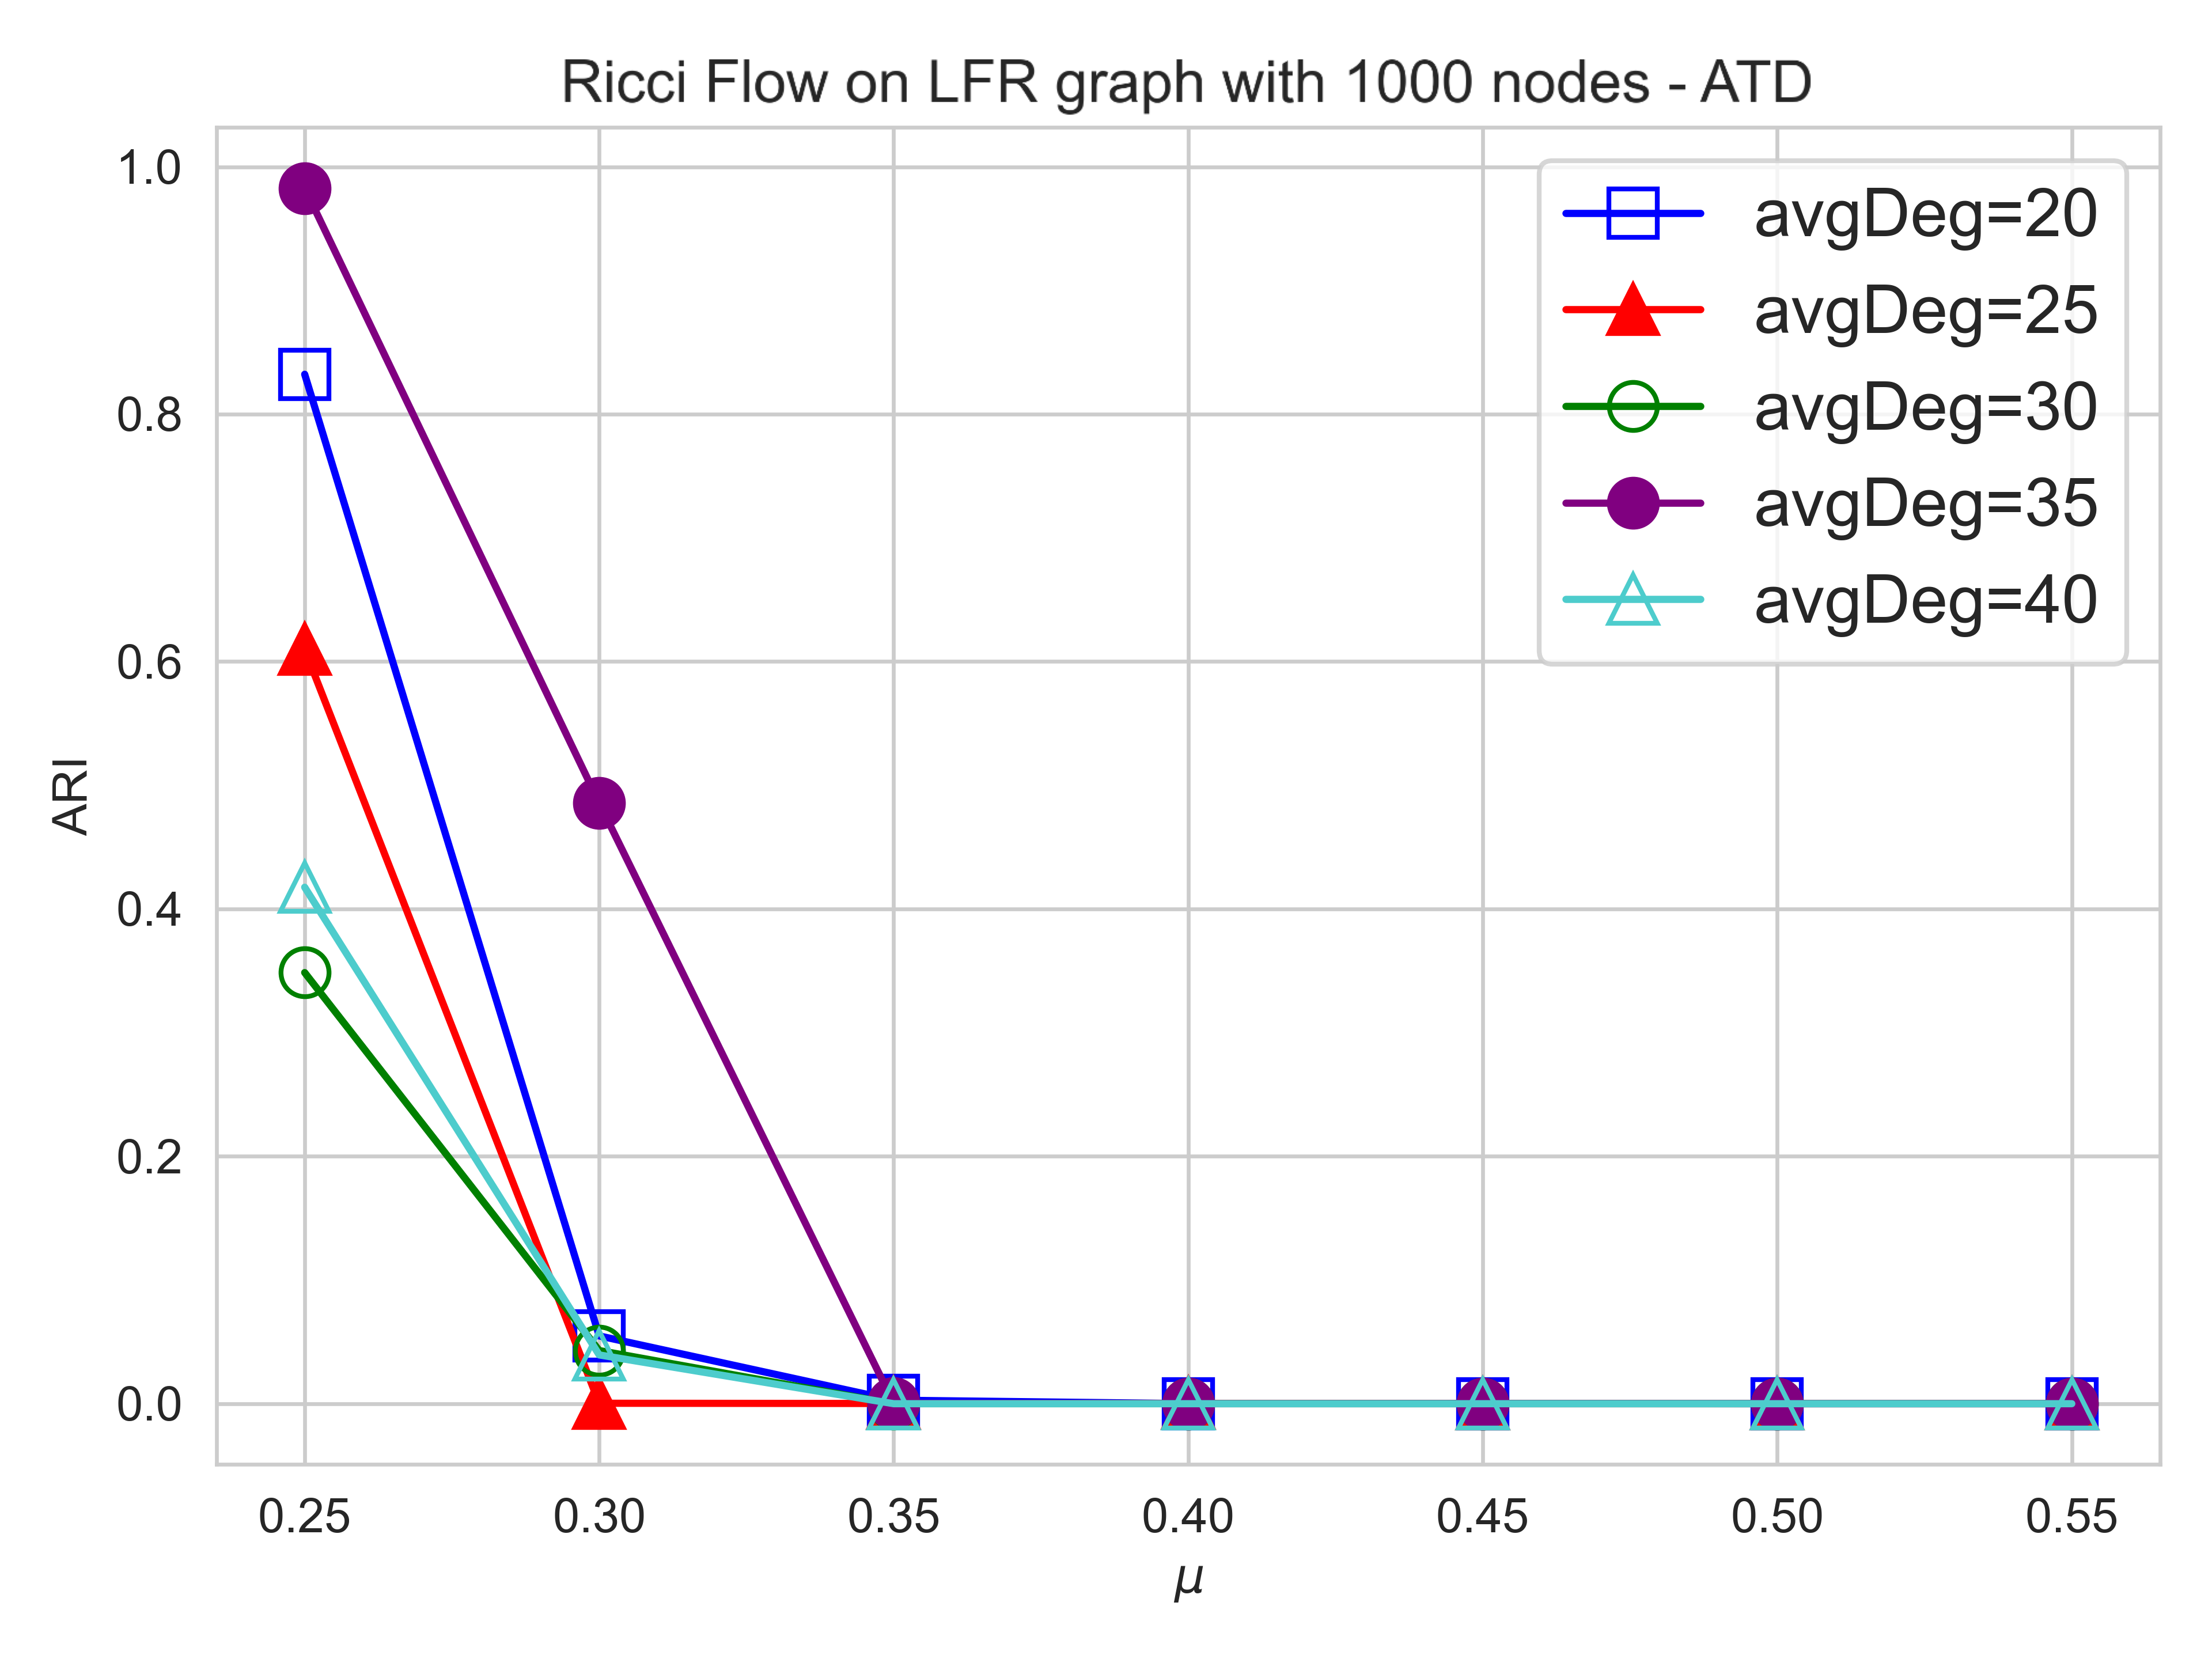
\includegraphics[width=0.6\textwidth]{../tests/LFRResults/LFR_ATD.png}
    \caption{LFR ATD.}
    \label{fig:LFR_ATD}
\end{figure}

Our graphs do not match exactly the plots of Ni et al., as for them the loss of ARI starts from higher values of $\mu$. This could be for various reasons:
\begin{itemize}
    \item It is unclear which parameter they used to generate LFR graphs. For example, using Networkx it is not possible to control exactly the number of communities (only a minimum and maximum number can be set), so they probably generated their graphs differently, fixing some parameters we did not have complete control on.
    \item They used an average ARI, probably generating the same graph multiple times. We generated the graph and applied the Ricci Flow just once due to an already high execution time.
    \item Their surgery process is not specified in detail. They might have used multiple surgeries over the same Ricci Flow process to remove possible singularities affecting the final performance (even though this should not be the case for this kind of graph).
\end{itemize}